\documentclass[12pt]{article} 
% \documentclass[12pt]{amsart} 

% Custom definitions
% To use this customization file, insert the line "% Custom definitions
% To use this customization file, insert the line "% Custom definitions
% To use this customization file, insert the line "\input{custom}" in the header of the tex file.

% Formatting

\tolerance=1000
\usepackage[margin=1in]{geometry}


% Packages

% \usepackage{amssymb,latexsym}
\usepackage{amssymb,amsfonts,amsmath,latexsym,amsthm}
\usepackage[usenames,dvipsnames]{color}
\usepackage[]{graphicx}
\usepackage[space]{grffile}
\usepackage{mathrsfs}   % fancy math font
% \usepackage[font=small,skip=0pt]{caption}
\usepackage[skip=0pt]{caption}
\usepackage{subcaption}
\usepackage{verbatim}
\usepackage{url}
\usepackage{bm}
\usepackage{dsfont}
\usepackage{extarrows}
\usepackage{multirow}
% \usepackage{wrapfig}
% \usepackage{epstopdf}
\usepackage{rotating}
\usepackage{tikz}
\usetikzlibrary{fit}					% fitting shapes to coordinates
%\usetikzlibrary{backgrounds}	% drawing the background after the foreground

\usepackage{fancyhdr}

\fancypagestyle{firststyle}{
   \fancyhf{}
   \renewcommand{\footrulewidth}{0.4pt}
   \fancyfoot[L]{\footnotesize This work is licensed under a \href{http://creativecommons.org/licenses/by-nc-nd/4.0/}{Creative Commons BY-NC-ND 4.0 International License}.\\ Jeffrey W. Miller (2015). \textit{Lecture Notes on Bayesian Statistics}. Duke University, Durham, NC.}
}


% \usepackage[dvipdfm,colorlinks,citecolor=blue,linkcolor=blue,urlcolor=blue]{hyperref}
\usepackage[colorlinks,citecolor=blue,linkcolor=blue,urlcolor=blue]{hyperref}
%\usepackage{hyperref}
\usepackage[authoryear,round]{natbib}


%  Theorems, etc.

\theoremstyle{plain}
\newtheorem{theorem}{Theorem}[section]
\newtheorem{corollary}[theorem]{Corollary}
\newtheorem{lemma}[theorem]{Lemma}
\newtheorem{proposition}[theorem]{Proposition}
\newtheorem{condition}[theorem]{Condition}
% \newtheorem{conditions}[theorem]{Conditions}

\theoremstyle{definition}
\newtheorem{definition}[theorem]{Definition}
% \newtheorem*{unnumbered-definition}{Definition}
\newtheorem{example}[theorem]{Example}
\theoremstyle{remark}
\newtheorem*{remark}{Remark}
\numberwithin{equation}{section}



% Document-specific shortcuts
\newcommand{\btheta}{{\bm\theta}}
\newcommand{\bbtheta}{{\pmb{\bm\theta}}}

\newcommand{\commentary}[1]{\ifx\showcommentary\undefined\else \emph{#1}\fi}

\newcommand{\term}[1]{\textit{\textbf{#1}}}

% Math shortcuts

% Probability distributions
\DeclareMathOperator*{\Exp}{Exp}
\DeclareMathOperator*{\TExp}{TExp}
\DeclareMathOperator*{\Bernoulli}{Bernoulli}
\DeclareMathOperator*{\Beta}{Beta}
\DeclareMathOperator*{\Ga}{Gamma}
\DeclareMathOperator*{\TGamma}{TGamma}
\DeclareMathOperator*{\Poisson}{Poisson}
\DeclareMathOperator*{\Binomial}{Binomial}
\DeclareMathOperator*{\NormalGamma}{NormalGamma}
\DeclareMathOperator*{\InvGamma}{InvGamma}
\DeclareMathOperator*{\Cauchy}{Cauchy}
\DeclareMathOperator*{\Uniform}{Uniform}
\DeclareMathOperator*{\Gumbel}{Gumbel}
\DeclareMathOperator*{\Pareto}{Pareto}
\DeclareMathOperator*{\Mono}{Mono}
\DeclareMathOperator*{\Geometric}{Geometric}
\DeclareMathOperator*{\Wishart}{Wishart}

% Math operators
\DeclareMathOperator*{\argmin}{arg\,min}
\DeclareMathOperator*{\argmax}{arg\,max}
\DeclareMathOperator*{\Cov}{Cov}
\DeclareMathOperator*{\diag}{diag}
\DeclareMathOperator*{\median}{median}
\DeclareMathOperator*{\Vol}{Vol}

% Math characters
\newcommand{\R}{\mathbb{R}}
\newcommand{\Z}{\mathbb{Z}}
\newcommand{\E}{\mathbb{E}}
\renewcommand{\Pr}{\mathbb{P}}
\newcommand{\I}{\mathds{1}}
\newcommand{\V}{\mathbb{V}}

\newcommand{\A}{\mathcal{A}}
\newcommand{\C}{\mathcal{C}}
\newcommand{\D}{\mathcal{D}}
\newcommand{\Hcal}{\mathcal{H}}
\newcommand{\M}{\mathcal{M}}
\newcommand{\N}{\mathcal{N}}
\newcommand{\X}{\mathcal{X}}
\newcommand{\Zcal}{\mathcal{Z}}
\renewcommand{\P}{\mathcal{P}}

\newcommand{\T}{\mathtt{T}}
\renewcommand{\emptyset}{\varnothing}


% Miscellaneous commands
\newcommand{\iid}{\stackrel{\mathrm{iid}}{\sim}}
\newcommand{\matrixsmall}[1]{\bigl(\begin{smallmatrix}#1\end{smallmatrix} \bigr)}

\newcommand{\items}[1]{\begin{itemize} #1 \end{itemize}}

\newcommand{\todo}[1]{\emph{\textcolor{red}{(#1)}}}

\newcommand{\branch}[4]{
\left\{
	\begin{array}{ll}
		#1  & \mbox{if } #2 \\
		#3 & \mbox{if } #4
	\end{array}
\right.
}

% approximately proportional to
\def\app#1#2{%
  \mathrel{%
    \setbox0=\hbox{$#1\sim$}%
    \setbox2=\hbox{%
      \rlap{\hbox{$#1\propto$}}%
      \lower1.3\ht0\box0%
    }%
    \raise0.25\ht2\box2%
  }%
}
\def\approxprop{\mathpalette\app\relax}

% \newcommand{\approptoinn}[2]{\mathrel{\vcenter{
  % \offinterlineskip\halign{\hfil$##$\cr
    % #1\propto\cr\noalign{\kern2pt}#1\sim\cr\noalign{\kern-2pt}}}}}

% \newcommand{\approxpropto}{\mathpalette\approptoinn\relax}





" in the header of the tex file.

% Formatting

\tolerance=1000
\usepackage[margin=1in]{geometry}


% Packages

% \usepackage{amssymb,latexsym}
\usepackage{amssymb,amsfonts,amsmath,latexsym,amsthm}
\usepackage[usenames,dvipsnames]{color}
\usepackage[]{graphicx}
\usepackage[space]{grffile}
\usepackage{mathrsfs}   % fancy math font
% \usepackage[font=small,skip=0pt]{caption}
\usepackage[skip=0pt]{caption}
\usepackage{subcaption}
\usepackage{verbatim}
\usepackage{url}
\usepackage{bm}
\usepackage{dsfont}
\usepackage{extarrows}
\usepackage{multirow}
% \usepackage{wrapfig}
% \usepackage{epstopdf}
\usepackage{rotating}
\usepackage{tikz}
\usetikzlibrary{fit}					% fitting shapes to coordinates
%\usetikzlibrary{backgrounds}	% drawing the background after the foreground

\usepackage{fancyhdr}

\fancypagestyle{firststyle}{
   \fancyhf{}
   \renewcommand{\footrulewidth}{0.4pt}
   \fancyfoot[L]{\footnotesize This work is licensed under a \href{http://creativecommons.org/licenses/by-nc-nd/4.0/}{Creative Commons BY-NC-ND 4.0 International License}.\\ Jeffrey W. Miller (2015). \textit{Lecture Notes on Bayesian Statistics}. Duke University, Durham, NC.}
}


% \usepackage[dvipdfm,colorlinks,citecolor=blue,linkcolor=blue,urlcolor=blue]{hyperref}
\usepackage[colorlinks,citecolor=blue,linkcolor=blue,urlcolor=blue]{hyperref}
%\usepackage{hyperref}
\usepackage[authoryear,round]{natbib}


%  Theorems, etc.

\theoremstyle{plain}
\newtheorem{theorem}{Theorem}[section]
\newtheorem{corollary}[theorem]{Corollary}
\newtheorem{lemma}[theorem]{Lemma}
\newtheorem{proposition}[theorem]{Proposition}
\newtheorem{condition}[theorem]{Condition}
% \newtheorem{conditions}[theorem]{Conditions}

\theoremstyle{definition}
\newtheorem{definition}[theorem]{Definition}
% \newtheorem*{unnumbered-definition}{Definition}
\newtheorem{example}[theorem]{Example}
\theoremstyle{remark}
\newtheorem*{remark}{Remark}
\numberwithin{equation}{section}



% Document-specific shortcuts
\newcommand{\btheta}{{\bm\theta}}
\newcommand{\bbtheta}{{\pmb{\bm\theta}}}

\newcommand{\commentary}[1]{\ifx\showcommentary\undefined\else \emph{#1}\fi}

\newcommand{\term}[1]{\textit{\textbf{#1}}}

% Math shortcuts

% Probability distributions
\DeclareMathOperator*{\Exp}{Exp}
\DeclareMathOperator*{\TExp}{TExp}
\DeclareMathOperator*{\Bernoulli}{Bernoulli}
\DeclareMathOperator*{\Beta}{Beta}
\DeclareMathOperator*{\Ga}{Gamma}
\DeclareMathOperator*{\TGamma}{TGamma}
\DeclareMathOperator*{\Poisson}{Poisson}
\DeclareMathOperator*{\Binomial}{Binomial}
\DeclareMathOperator*{\NormalGamma}{NormalGamma}
\DeclareMathOperator*{\InvGamma}{InvGamma}
\DeclareMathOperator*{\Cauchy}{Cauchy}
\DeclareMathOperator*{\Uniform}{Uniform}
\DeclareMathOperator*{\Gumbel}{Gumbel}
\DeclareMathOperator*{\Pareto}{Pareto}
\DeclareMathOperator*{\Mono}{Mono}
\DeclareMathOperator*{\Geometric}{Geometric}
\DeclareMathOperator*{\Wishart}{Wishart}

% Math operators
\DeclareMathOperator*{\argmin}{arg\,min}
\DeclareMathOperator*{\argmax}{arg\,max}
\DeclareMathOperator*{\Cov}{Cov}
\DeclareMathOperator*{\diag}{diag}
\DeclareMathOperator*{\median}{median}
\DeclareMathOperator*{\Vol}{Vol}

% Math characters
\newcommand{\R}{\mathbb{R}}
\newcommand{\Z}{\mathbb{Z}}
\newcommand{\E}{\mathbb{E}}
\renewcommand{\Pr}{\mathbb{P}}
\newcommand{\I}{\mathds{1}}
\newcommand{\V}{\mathbb{V}}

\newcommand{\A}{\mathcal{A}}
\newcommand{\C}{\mathcal{C}}
\newcommand{\D}{\mathcal{D}}
\newcommand{\Hcal}{\mathcal{H}}
\newcommand{\M}{\mathcal{M}}
\newcommand{\N}{\mathcal{N}}
\newcommand{\X}{\mathcal{X}}
\newcommand{\Zcal}{\mathcal{Z}}
\renewcommand{\P}{\mathcal{P}}

\newcommand{\T}{\mathtt{T}}
\renewcommand{\emptyset}{\varnothing}


% Miscellaneous commands
\newcommand{\iid}{\stackrel{\mathrm{iid}}{\sim}}
\newcommand{\matrixsmall}[1]{\bigl(\begin{smallmatrix}#1\end{smallmatrix} \bigr)}

\newcommand{\items}[1]{\begin{itemize} #1 \end{itemize}}

\newcommand{\todo}[1]{\emph{\textcolor{red}{(#1)}}}

\newcommand{\branch}[4]{
\left\{
	\begin{array}{ll}
		#1  & \mbox{if } #2 \\
		#3 & \mbox{if } #4
	\end{array}
\right.
}

% approximately proportional to
\def\app#1#2{%
  \mathrel{%
    \setbox0=\hbox{$#1\sim$}%
    \setbox2=\hbox{%
      \rlap{\hbox{$#1\propto$}}%
      \lower1.3\ht0\box0%
    }%
    \raise0.25\ht2\box2%
  }%
}
\def\approxprop{\mathpalette\app\relax}

% \newcommand{\approptoinn}[2]{\mathrel{\vcenter{
  % \offinterlineskip\halign{\hfil$##$\cr
    % #1\propto\cr\noalign{\kern2pt}#1\sim\cr\noalign{\kern-2pt}}}}}

% \newcommand{\approxpropto}{\mathpalette\approptoinn\relax}





" in the header of the tex file.

% Formatting

\tolerance=1000
\usepackage[margin=1in]{geometry}


% Packages

% \usepackage{amssymb,latexsym}
\usepackage{amssymb,amsfonts,amsmath,latexsym,amsthm}
\usepackage[usenames,dvipsnames]{color}
\usepackage[]{graphicx}
\usepackage[space]{grffile}
\usepackage{mathrsfs}   % fancy math font
% \usepackage[font=small,skip=0pt]{caption}
\usepackage[skip=0pt]{caption}
\usepackage{subcaption}
\usepackage{verbatim}
\usepackage{url}
\usepackage{bm}
\usepackage{dsfont}
\usepackage{extarrows}
\usepackage{multirow}
% \usepackage{wrapfig}
% \usepackage{epstopdf}
\usepackage{rotating}
\usepackage{tikz}
\usetikzlibrary{fit}					% fitting shapes to coordinates
%\usetikzlibrary{backgrounds}	% drawing the background after the foreground

\usepackage{fancyhdr}

\fancypagestyle{firststyle}{
   \fancyhf{}
   \renewcommand{\footrulewidth}{0.4pt}
   \fancyfoot[L]{\footnotesize This work is licensed under a \href{http://creativecommons.org/licenses/by-nc-nd/4.0/}{Creative Commons BY-NC-ND 4.0 International License}.\\ Jeffrey W. Miller (2015). \textit{Lecture Notes on Bayesian Statistics}. Duke University, Durham, NC.}
}


% \usepackage[dvipdfm,colorlinks,citecolor=blue,linkcolor=blue,urlcolor=blue]{hyperref}
\usepackage[colorlinks,citecolor=blue,linkcolor=blue,urlcolor=blue]{hyperref}
%\usepackage{hyperref}
\usepackage[authoryear,round]{natbib}


%  Theorems, etc.

\theoremstyle{plain}
\newtheorem{theorem}{Theorem}[section]
\newtheorem{corollary}[theorem]{Corollary}
\newtheorem{lemma}[theorem]{Lemma}
\newtheorem{proposition}[theorem]{Proposition}
\newtheorem{condition}[theorem]{Condition}
% \newtheorem{conditions}[theorem]{Conditions}

\theoremstyle{definition}
\newtheorem{definition}[theorem]{Definition}
% \newtheorem*{unnumbered-definition}{Definition}
\newtheorem{example}[theorem]{Example}
\theoremstyle{remark}
\newtheorem*{remark}{Remark}
\numberwithin{equation}{section}



% Document-specific shortcuts
\newcommand{\btheta}{{\bm\theta}}
\newcommand{\bbtheta}{{\pmb{\bm\theta}}}

\newcommand{\commentary}[1]{\ifx\showcommentary\undefined\else \emph{#1}\fi}

\newcommand{\term}[1]{\textit{\textbf{#1}}}

% Math shortcuts

% Probability distributions
\DeclareMathOperator*{\Exp}{Exp}
\DeclareMathOperator*{\TExp}{TExp}
\DeclareMathOperator*{\Bernoulli}{Bernoulli}
\DeclareMathOperator*{\Beta}{Beta}
\DeclareMathOperator*{\Ga}{Gamma}
\DeclareMathOperator*{\TGamma}{TGamma}
\DeclareMathOperator*{\Poisson}{Poisson}
\DeclareMathOperator*{\Binomial}{Binomial}
\DeclareMathOperator*{\NormalGamma}{NormalGamma}
\DeclareMathOperator*{\InvGamma}{InvGamma}
\DeclareMathOperator*{\Cauchy}{Cauchy}
\DeclareMathOperator*{\Uniform}{Uniform}
\DeclareMathOperator*{\Gumbel}{Gumbel}
\DeclareMathOperator*{\Pareto}{Pareto}
\DeclareMathOperator*{\Mono}{Mono}
\DeclareMathOperator*{\Geometric}{Geometric}
\DeclareMathOperator*{\Wishart}{Wishart}

% Math operators
\DeclareMathOperator*{\argmin}{arg\,min}
\DeclareMathOperator*{\argmax}{arg\,max}
\DeclareMathOperator*{\Cov}{Cov}
\DeclareMathOperator*{\diag}{diag}
\DeclareMathOperator*{\median}{median}
\DeclareMathOperator*{\Vol}{Vol}

% Math characters
\newcommand{\R}{\mathbb{R}}
\newcommand{\Z}{\mathbb{Z}}
\newcommand{\E}{\mathbb{E}}
\renewcommand{\Pr}{\mathbb{P}}
\newcommand{\I}{\mathds{1}}
\newcommand{\V}{\mathbb{V}}

\newcommand{\A}{\mathcal{A}}
\newcommand{\C}{\mathcal{C}}
\newcommand{\D}{\mathcal{D}}
\newcommand{\Hcal}{\mathcal{H}}
\newcommand{\M}{\mathcal{M}}
\newcommand{\N}{\mathcal{N}}
\newcommand{\X}{\mathcal{X}}
\newcommand{\Zcal}{\mathcal{Z}}
\renewcommand{\P}{\mathcal{P}}

\newcommand{\T}{\mathtt{T}}
\renewcommand{\emptyset}{\varnothing}


% Miscellaneous commands
\newcommand{\iid}{\stackrel{\mathrm{iid}}{\sim}}
\newcommand{\matrixsmall}[1]{\bigl(\begin{smallmatrix}#1\end{smallmatrix} \bigr)}

\newcommand{\items}[1]{\begin{itemize} #1 \end{itemize}}

\newcommand{\todo}[1]{\emph{\textcolor{red}{(#1)}}}

\newcommand{\branch}[4]{
\left\{
	\begin{array}{ll}
		#1  & \mbox{if } #2 \\
		#3 & \mbox{if } #4
	\end{array}
\right.
}

% approximately proportional to
\def\app#1#2{%
  \mathrel{%
    \setbox0=\hbox{$#1\sim$}%
    \setbox2=\hbox{%
      \rlap{\hbox{$#1\propto$}}%
      \lower1.3\ht0\box0%
    }%
    \raise0.25\ht2\box2%
  }%
}
\def\approxprop{\mathpalette\app\relax}

% \newcommand{\approptoinn}[2]{\mathrel{\vcenter{
  % \offinterlineskip\halign{\hfil$##$\cr
    % #1\propto\cr\noalign{\kern2pt}#1\sim\cr\noalign{\kern-2pt}}}}}

% \newcommand{\approxpropto}{\mathpalette\approptoinn\relax}






\setcounter{tocdepth}{2}

\graphicspath{{figures/}}

\title{Chapter 1: Foundations}
\author{}
\date{}

\def\showcommentary{1}


\begin{document}
\maketitle
{\footnotesize
\tableofcontents 
}
\thispagestyle{firststyle}

\newpage

\section{How random is the flip of a coin?}

\subsection{``It's a toss-up''}
\begin{itemize}
\item It is so generally assumed that a coin toss comes up heads half of the time, that it has even become a standard metaphor for two events with equal probability.
\item But think about it---is it really 50-50? Suppose we always flip a coin starting with heads up. Could the outcome actually be biased toward either heads or tails?
\item Assume the coin is physically symmetric. Since an ``in-flight'' coin is a relatively simple physical system, the outcome should be essentially determined by the initial conditions at the beginning of it's trajectory. So, any randomness comes from the flipper, not the flipping.
% \item We could test this with an experiment. First, let's make our assumptions clear.
\item Experiment: Flip a coin $n = 10$ times, starting with heads up each time. (flip, flip, flip, \dots) Do we know anything more now than when we started? We got some data, so we should know more now. But probably we need more data! How much more? How can we quantify our uncertainty about the answer?
\item (And now comes the surprise: Diaconis et al.\ (2007) argue that, in fact, the outcome is slightly biased due to precession, and will come up the same way it started about 51\% of the time!  This is based on physical, rather than statistical, evidence.)
\end{itemize}

\subsection{Probability and Statistics are two sides of the same coin}
\begin{itemize}
\item Let $X_1,\dotsc,X_n$ be the outcomes of $n$ coin flips, and suppose they are i.i.d.\ (independent and identically distributed), with the probability of heads equal to $\theta$.
\item This defines a probabilistic model, for which---if we knew $\theta$---we could prove all kinds of things about the distribution of $X_{1:n} = (X_1,\dotsc,X_n)$. This is Probability.
\item Statistics, meanwhile, goes the other direction---trying to obtain information about $\theta$ from $X_{1:n}$.
\begin{alignat*}{2}
&\text{Probability: } \qquad && \theta\longrightarrow X_{1:n} \\
&\text{Statistics: } \qquad && \theta\longleftarrow X_{1:n}
\end{alignat*}
% \item One could say that probability is deductive, while statistics is inductive.
\item To see if the outcome is biased, based on the data $X_1,\dotsc,X_n$, perhaps the first thing that comes to mind is to simply look at the proportion of heads, and see if it's close to $1/2$. But on reflection, there are some issues with this:
\begin{itemize}
\item How close is ``close''?
\item How would we quantify our uncertainty about the correct answer?
\item If $n$ is very small, say 2 or 3, there is a good chance that the flips will all come up the same (all heads or all tails), in which case the proportion of heads would be 1 or 0. But from experience, we know $\theta$ is unlikely to be close to 1 or 0. Would it be better to take such prior knowledge into account?
\end{itemize}
\end{itemize}

\subsection{The Bayesian approach}

\begin{figure}
    \centering
    \begin{subfigure}[t]{0.33\textwidth}
        \centering
        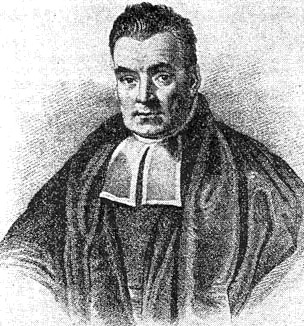
\includegraphics[height=2in]{Bayes.jpg}
        % Source: http://commons.wikimedia.org/wiki/File:Thomas_Bayes.gif
        % License: This work is in the public domain in the United States, and those countries with a copyright term of life of the author plus 100 years or less.
        % Date accessed: 12/28/2014
        \caption*{$\Pr(\text{this}=\text{Bayes}\mid \text{data}) < 1$}
    \end{subfigure}%
    ~ 
    \begin{subfigure}[t]{0.33\textwidth}
        \centering
        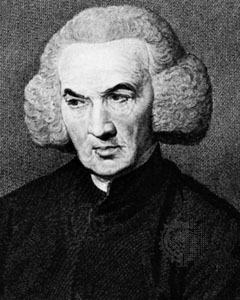
\includegraphics[height=2in]{Price.jpg}
        % Source: http://commons.wikimedia.org/wiki/File:Richard_Price.jpg
        % License: This work is in the public domain in the United States, and those countries with a copyright term of life of the author plus 100 years or less.
        % Date accessed: 12/28/2014        
        \caption*{Richard Price}
    \end{subfigure}%
    ~
    \begin{subfigure}[t]{0.33\textwidth}
        \centering
        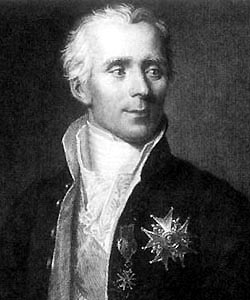
\includegraphics[height=2in]{Laplace.jpg}
        % Source: http://commons.wikimedia.org/wiki/File:Pierre-Simon-Laplace_(1749-1827).jpg
        % License: (POSSIBLE ISSUES WITH LICENSE --- SEE SOURCE) This image (or other media file) is in the public domain because its copyright has expired. This applies to Australia, the European Union and those countries with a copyright term of life of the author plus 70 years. 
        % Date accessed: 12/28/2014
        \caption*{Pierre-Simon Laplace}
    \end{subfigure}
    \caption{Founders of Bayesian statistics.}
    \label{figure:founders}
\end{figure}

\begin{itemize}
    \item Thomas Bayes (1701?--1761) was an ordained minister who was also a talented mathematician and a Fellow of the Royal Society.  Bayes came up with an ingenious solution to this problem, but died before publishing it. Fortunately, his friend Richard Price carried his work further and published it in 1764. Apparently independently, Laplace rediscovered essentially the same idea in 1774, and developed it much further. (See Figure \ref{figure:founders}.)
\item The idea is to assume a \term{prior} probability distribution for $\theta$---that is, a distribution representing the plausibility of each possible value of $\theta$ before the data is observed. Then, to make inferences about $\theta$, one simply considers the conditional distribution of $\theta$ given the observed data. This is referred to as the \term{posterior} distribution, since it represents the plausibility of each possible value of $\theta$ after seeing the data.
\item Mathematically, this is expressed via \term{Bayes' theorem},
\begin{align}\label{equation:Bayes}
% p(\theta|x_{1:n}) =\frac{p(x_{1:n}|\theta) p(\theta)}{p(x_{1:n})}\propto p(x_{1:n}|\theta) p(\theta),
p(\theta|x) =\frac{p(x|\theta) p(\theta)}{p(x)}\propto p(x|\theta) p(\theta),
\end{align}
where $x$ is the observed data (for example, $x = x_{1:n}$). In words, we say ``the posterior is proportional to the likelihood times the prior''. Bayes' theorem is essentially just the definition of conditional probability
$$\Pr(B|A) =\frac{\Pr(A\cap B)}{\Pr(A)} =\frac{\Pr(A|B)\Pr(B)}{\Pr(A)} $$
extended to conditional densities. (From the modern perspective, Bayes' theorem is a trivial consequence of the definition of a conditional density---however, when Bayes wrote his paper, the idea of a conditional probability density did not yet exist!)
\item More generally, the Bayesian approach---in a nutshell---is to assume a prior distribution on any unknowns, and then just follow the rules of probability to answer any questions of interest. This provides a coherent framework for making inferences about unknown parameters $\theta$ as well as any future data or missing data, and for making rational decisions based on such inferences. 
\end{itemize}


%\newpage

\section{Beta-Bernoulli model}
\label{section:Beta-Bernoulli}

We now formally explore a Bayesian approach to the coin flipping problem.

\begin{figure}
  \begin{center}
    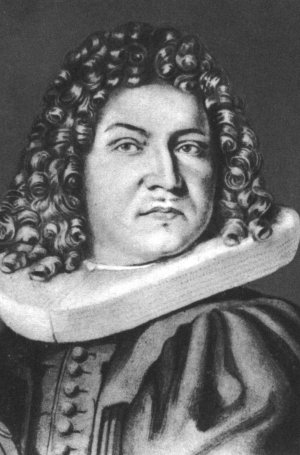
\includegraphics[width=0.25\textwidth]{Bernoulli.jpg}
    % Source: http://commons.wikimedia.org/wiki/File:Jakob_Bernoulli.jpg
    % License: (POSSIBLE ISSUES WITH LICENSE --- SEE SOURCE) This image (or other media file) is in the public domain because its copyright has expired. This applies to Australia, the European Union and those countries with a copyright term of life of the author plus 70 years. 
    % Date accessed: 12/28/2014
  \end{center}
  \caption{Jacob Bernoulli (not in a bad mood, everyone is just annoying).}
\end{figure}

\subsection{Bernoulli distribution}
\begin{itemize}
\item The Bernoulli distribution models binary outcomes, i.e., taking two possible values. The convention is to use $0$ and $1$.
\item It is named for Jacob Bernoulli (1655--1705), who is known for various inconsequential trivialities such as developing the foundations of 
probability theory (including the law of large numbers), 
combinatorics,
differential equations, and
the calculus of variations.
Oh, and he discovered the constant $e$.
\item The Bernoulli distribution shows up everywhere, due to the ubiquity of binary outcomes (for instance, in computer vision, neuroscience, demographics and polling, public health and epidemiology, etc. etc. etc.).
\item We write $X\sim\Bernoulli(\theta)$ to mean that
$$\Pr(X = x\mid\theta) = \branch{\theta}{x = 1}{1-\theta}{x = 0}$$
and is $0$ otherwise.  In other words, the p.m.f.\ (probability mass function) is
$$ p(x|\theta) =\Pr(X = x\mid\theta) = \theta^x(1-\theta)^{1-x} \I(x\in\{0,1\}).$$
\item The mean (or expectation) is $\E X =\sum_{x\in\{0,1\}} x p(x|\theta) =\theta$.
\item Notation: $\Pr$ denotes ``the probability of'', and $\E$ denotes the expectation. The \term{indicator function}, $\I(E)$, equals $1$ when $E$ is true and is $0$ otherwise. The symbol $\in$ means ``belongs to the set''.
\item If $X_1,\dotsc,X_n\iid\Bernoulli(\theta)$ then for $x_1,\dotsc,x_n\in\{0,1\}$,
\begin{align}
p(x_{1:n}|\theta) &= \Pr(X_1 = x_1,\dotsc,X_n = x_n\mid\theta) \notag\\
& =\prod_{i = 1}^n \Pr(X_i = x_i\mid\theta) \notag\\
& = \prod_{i = 1}^n p(x_i|\theta) \notag\\
& =\prod_{i = 1}^n \theta^{x_i}(1-\theta)^{1-x_i} \notag\\
& =\theta^{\sum x_i}(1-\theta)^{n-\sum x_i}. \label{equation:likelihood}
\end{align}
\item Viewed as a function of $\theta$, $p(x_{1:n}|\theta)$ is called the \term{likelihood function}. It is sometimes denoted $L(\theta; x_{1:n})$ to emphasize this. Viewed as a distribution on $x_{1:n}$, we will refer to this as the \term{generator} or \term{generating distribution} (sometimes it is referred to as the ``sampling distribution'', but this becomes ambiguous when one is also sampling from the posterior).
\end{itemize}

\subsection{Beta distribution}

\begin{figure}
  \begin{center}
    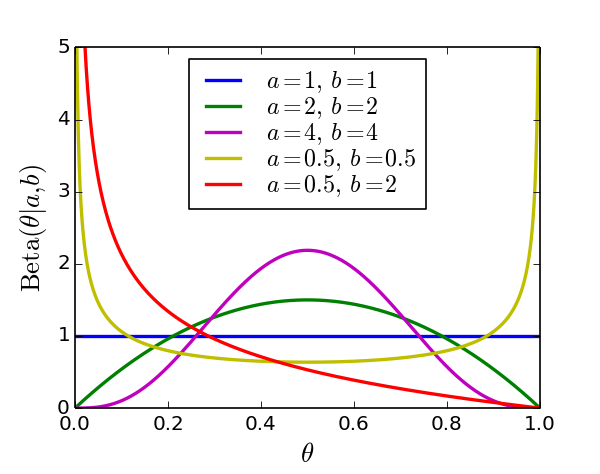
\includegraphics[width=0.6\textwidth]{Beta.png}
    % Source: Original work by Jeffrey W. Miller.
  \end{center}
  \caption{Some Beta p.d.f.s.}
\end{figure}


\begin{itemize}
\item Bayes used a uniform prior on $\theta$, which is a special case of the beta distribution.
\item Given $a,b>0$, we write $\btheta\sim\Beta(a,b)$ to mean $\btheta$ has p.d.f.\ (probability density function)
\begin{align}\label{equation:beta}
p(\theta) =\Beta(\theta|a,b) =\frac{1}{B(a,b)}\theta^{a-1}(1-\theta)^{b-1}\I(0<\theta<1),
\end{align}
i.e., $p(\theta)\propto \theta^{a-1}(1-\theta)^{b-1}$ on the interval from $0$ to $1$. Here, $B(a,b)$ is Euler's beta function.
\item The mean is $\E\,\btheta =\int \theta\,p(\theta)d\theta = a/(a+b)$.
\end{itemize}

\subsubsection*{Notation}
\begin{itemize}
\item $f(x)\propto g(x)$ (``$f$ is proportional to $g$'') means there is a constant $c$ such that $f(x) = c g(x)$ for all $x$. For functions of multiple variables, say $x$ and $y$, we write $\underset{x}{\propto}$ to indicate proportionality with respect to $x$ only. This simple device is surprisingly useful for deriving posterior distributions.
\item Usually, we use capital letters to denote random variables (e.g., $X$) and lowercase for particular values (e.g., $x$). However, in the case of theta, we will use bold font to denote the random variable $\btheta$, and unbold for particular values $\theta$.
\item We will usually use $p$ for all p.d.f.s and p.m.f.s, following the usual convention that the symbol used (e.g., the $\theta$ in the expression $p(\theta)$) indicates which random variable we are talking about.
\end{itemize}


\subsection{The posterior}

\begin{figure}
  \begin{center}
    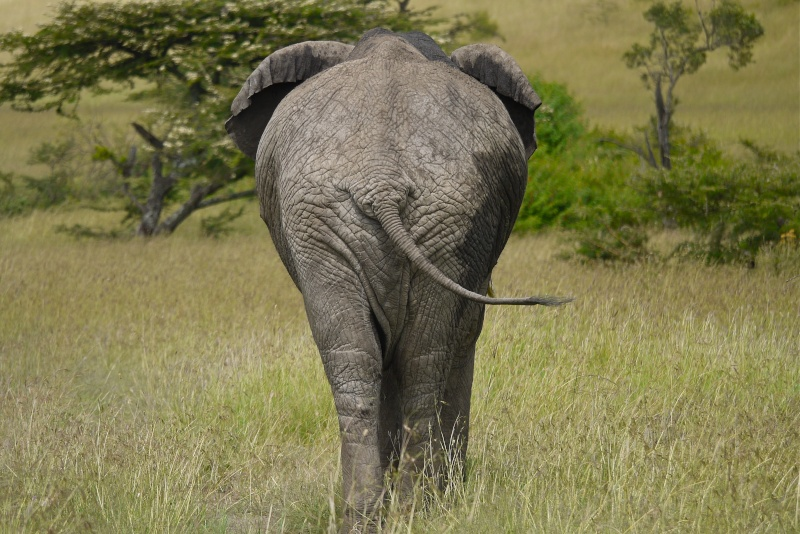
\includegraphics[width=0.5\textwidth]{elephant-posterior.jpg}
    % Source: http://wildaboutanimals.forumotion.net/t1808-elephants-of-the-mara-june-2012
    %         http://i33.servimg.com/u/f33/17/63/41/49/p1030711.jpg
    %         "Safariman", Buckinghamshire
    % License: UNKNOWN
    % Date accessed: 12/28/2014
  \end{center}
  \caption*{A posteriori}
\end{figure}

\begin{itemize}
\item Using Bayes' theorem (Equation \ref{equation:Bayes}), and plugging in the likelihood (Equation \ref{equation:likelihood}) and the prior (Equation \ref{equation:beta}), the posterior is
\begin{align}
p(\theta|x_{1:n}) &\propto p(x_{1:n}|\theta) p(\theta)\notag\\
& =\theta^{\sum x_i}(1-\theta)^{n-\sum x_i}\frac{1}{B(a,b)}\theta^{a-1}(1-\theta)^{b-1}\I(0<\theta<1) \notag\\
& \propto \theta^{a +\sum x_i - 1}(1-\theta)^{b +n-\sum x_i - 1}\I(0<\theta<1)\notag\\
& \propto \textstyle\Beta\big(\theta\mid a +\sum x_i, \, b + n-\sum x_i\big).
\label{equation:Beta-Bernoulli-posterior}
\end{align}
\item So, the posterior has the same form (a Beta distribution) as the prior! When this happens, we say that the prior is \term{conjugate} (more on this later).
\item Since the posterior has such a nice form, it is easy to work with---e.g., for computing certain integrals with respect to the posterior, sampling from the posterior, and computing the posterior p.d.f.\ and its derivatives.
\end{itemize}

\subsubsection*{Example}
\begin{itemize}
\item Suppose we choose $a = 1$ and $b = 1$, so that the prior is uniform.  As a simulation to see how the posterior behaves, let's generate data $X_1,\dotsc,X_n\iid\Bernoulli(\theta_0)$ with $\theta_0 = 0.51$.
\item Figure \ref{figure:posterior} shows the posterior p.d.f.\ for increasing amounts of data. (Note that this will be different each time the experiment is run, because the samples will be different.)
\end{itemize}

\begin{figure}
  \begin{center}
    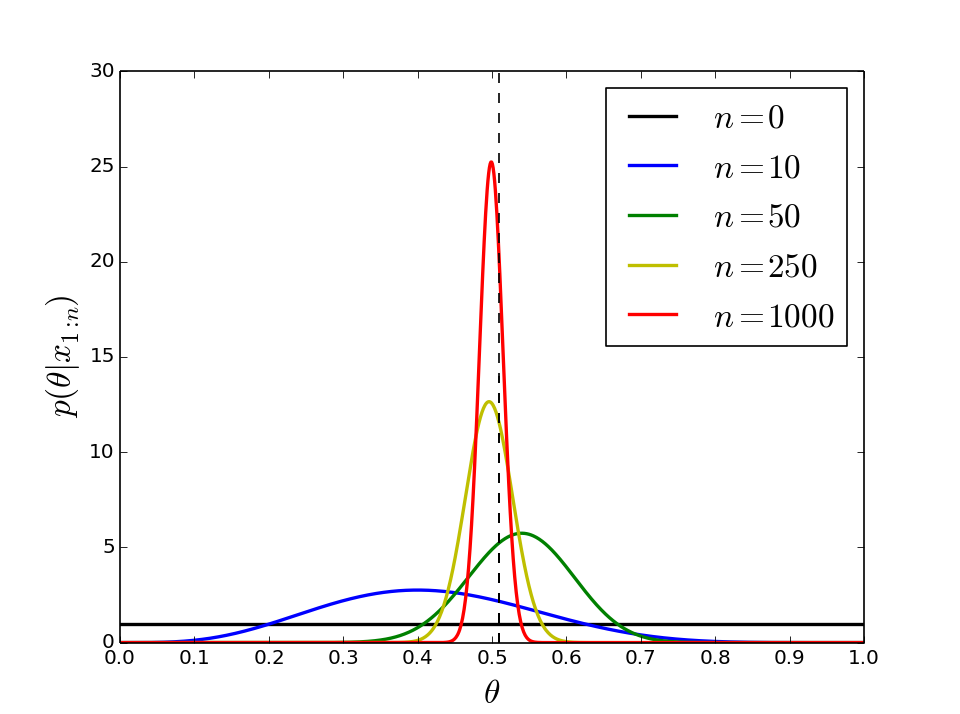
\includegraphics[width=0.8\textwidth]{posterior.png}
    % Source: Original work of Jeffrey W. Miller.
  \end{center}
  \caption{Posterior densities. The dotted line shows the true value of theta.}
  \label{figure:posterior}
\end{figure}




\newpage

\section{The cast of characters}

Here's a list of the mathematical objects we will most frequently encounter. So far, we've seen the likelihood, prior, and posterior. In the rest of this chapter, we will get acquainted with the rest of them. Here, we denote the observed data by $x$, noting that this may consist of many data points, e.g., $x = x_{1:n}=(x_1,\dotsc,x_n)$.

\begin{center}
\begin{tabular}{ l l }
generator / likelihood & $p(x|\theta)$  \\
prior & $p(\theta)$ \\
posterior & $p(\theta|x)$ \\
marginal likelihood & $p(x)$ \\
posterior predictive & $p(x_{n+1}|x_{1:n})$ \\
loss function & $\ell(s,a)$ \\
posterior expected loss & $\rho(a,x)$ \\
risk / frequentist risk & $R(\theta,\delta)$ \\
integrated risk & $r(\delta)$
\end{tabular}
\end{center}

\subsection{Marginal likelihood and posterior predictive}

The \term{marginal likelihood} is 
$$ p(x) = \int p(x|\theta) p(\theta) \,d\theta $$
i.e., it is the marginal p.d.f./p.m.f.\ of the observed data, obtained by integrating $\theta$ out of the joint density $p(x,\theta) = p(x|\theta) p(\theta)$. When $\theta$ is a vector, this will be a multi-dimensional integral.

When the data is a sequence $x =(x_1,\dotsc,x_n)$, the \term{posterior predictive distribution} is the distribution of $X_{n+1}$ given $X_{1:n}= x_{1:n}$.  When $X_1,\dotsc,X_n,X_{n+1}$ are independent given $\btheta =\theta$, the posterior predictive p.d.f./p.m.f.\ is given by
\begin{align*}
p(x_{n+1}|x_{1:n}) &= \int p(x_{n+1},\theta|x_{1:n})\,d\theta\\
&= \int p(x_{n+1}|\theta,x_{1:n}) p(\theta|x_{1:n})\,d\theta\\
& = \int p(x_{n+1}|\theta) p(\theta|x_{1:n})\,d\theta.
\end{align*}

\subsection{Example: Beta-Bernoulli}

If $\btheta\sim\Beta(a,b)$ and $X_1,\dotsc,X_n\mid \btheta =\theta$ are i.i.d.\ $\Bernoulli(\theta)$ (as in Section \ref{section:Beta-Bernoulli}), then the marginal likelihood is
\begin{align*}
p(x_{1:n}) &= \int p(x_{1:n}|\theta) p(\theta) \,d\theta\\
& = \int_0^1\theta^{\sum x_i}(1-\theta)^{n-\sum x_i}\frac{1}{B(a,b)}\theta^{a-1}(1-\theta)^{b-1} d\theta\\
& =\frac{B\big(a +\sum x_i,\, b + n-\sum x_i\big)}{B(a,b)},
\end{align*}
by the integral definition of the Beta function.
Letting $a_n = a +\sum x_i$ and $b_n = b + n-\sum x_i$ for brevity, and using the fact (from Equation \ref{equation:Beta-Bernoulli-posterior}) that $p(\theta|x_{1:n}) = \Beta(\theta|a_n,b_n)$,
\begin{align*}
\Pr(X_{n+1} = 1\mid x_{1:n}) & = \int \Pr(X_{n+1} = 1\mid \theta) p(\theta|x_{1:n}) d\theta\\
& =\int \theta\,\Beta(\theta|a_n,b_n) =\frac{a_n}{a_n + b_n},
\end{align*}
hence, the posterior predictive p.m.f.\ is
\begin{align*}
p(x_{n+1}|x_{1:n}) & = \frac{a_n^{x_{n+1}} b_n^{1-x_{n+1}}}{a_n + b_n}\I(x_{n+1}\in\{0,1\}).
\end{align*}



%\newpage
\vspace{10ex}

\section{Decision theory}

\begin{figure}
    \centering
    \begin{subfigure}[t]{0.5\textwidth}
        \centering
        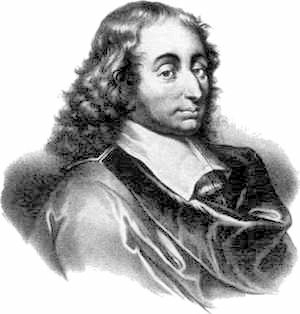
\includegraphics[height=2in]{Pascal.jpg}
        % Source: http://commons.wikimedia.org/wiki/File:Blaise_pascal.jpg
        % License: (POSSIBLE ISSUES WITH LICENSE --- SEE SOURCE) This image (or other media file) is in the public domain because its copyright has expired. This applies to Australia, the European Union and those countries with a copyright term of life of the author plus 70 years. 
        % Date accessed: 12/31/2014
        \caption*{Blaise Pascal}
    \end{subfigure}%
    ~ 
    \begin{subfigure}[t]{0.5\textwidth}
        \centering
        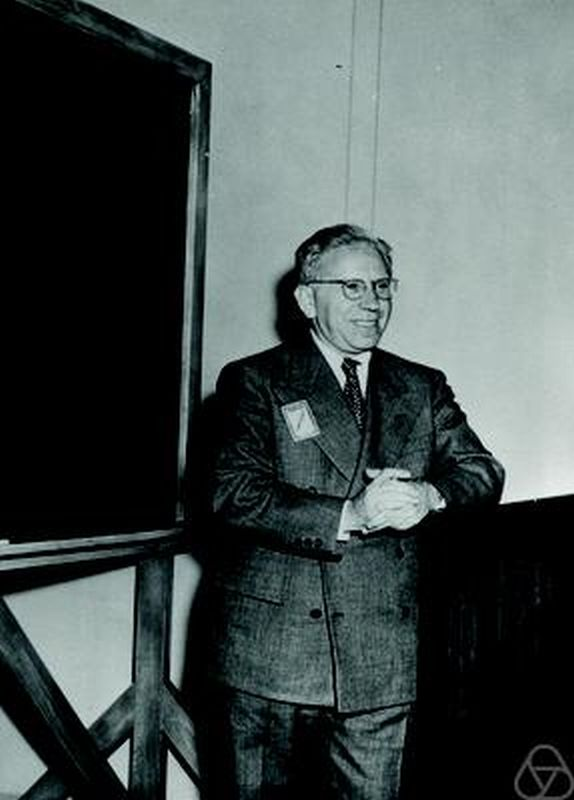
\includegraphics[height=3in]{Wald.jpg}
        % Source: http://commons.wikimedia.org/wiki/File:Abraham_Wald.jpg
        % License: This file is licensed under the Creative Commons Attribution-Share Alike 2.0 Germany license.
        % ("... The above applies to the Work as incorporated in a Collective Work, but this does not require the Collective Work apart from the Work itself to be made subject to the terms of this License.")
        % Date accessed: 12/31/2014        
        \caption*{Abraham Wald}
    \end{subfigure}
    \caption{Historical figures in decision theory.}
\end{figure}


In decision theory, we start with the end in mind---how are we actually going to use our inferences and what consequences will this have? The basic goal is to minimize loss (or equivalently, to maximize utility/gain). While there are multiple ways of making this precise, here we consider the standard Bayesian approach, which is to minimize posterior expected loss.

A famous early example of decision-theoretic reasoning is Pascal's Wager, in which Blaise Pascal (1623--1662) suggested the following argument for believing in God: If God exists then one will reap either an infinite gain or infinite loss (eternity in heaven or hell), depending on whether one believes or not---meanwhile, if he does not exist, the gain or loss is finite. Thus, he reasoned, no matter how small the probability that God exists, the rational decision is to believe. Pascal's loss function can be represented by the following matrix, in which $1$ indicates existence, $0$ indicates non-existence, and $\alpha,\beta$ are finite values:

\begin{center}
\begin{tabular}{l r|c|c|}
\multicolumn{2}{r}{} & \multicolumn{2}{c}{Belief} \\
\multicolumn{2}{r}{}
 &  \multicolumn{1}{c}{$0$}
 & \multicolumn{1}{c}{$1$} \\
\cline{3-4}
\multirow{2}{*}{Truth} 
   & $0$ & $\alpha$ & $\beta$ \\
   \cline{3-4}
   & $1$ & $\infty$ & $-\infty$ \\
   \cline{3-4}
\end{tabular}
\end{center}

In statistics, loss functions were used in a limited way during the 1700s and 1800s (most notably Laplace's absolute error and Gauss' quadratic error), but the real developments would have to wait until the 1900s.

The father of statistical decision theory was Abraham Wald (1902--1950). Wald was born in Austria-Hungary, and moved to the United States after the annexation of Austria into Germany in 1938. In 1939, he published a groundbreaking paper establishing the foundations of modern statistical decision theory. Wald also developed sequential analysis, made significant contributions to econometrics and geometry, and provided an important statistical analysis of aircraft vulnerability during World War II.

\subsection{The basics of Bayesian decision theory}

\begin{itemize}
\item The general setup is that there is some unknown state $S$ (a.k.a. the state of nature), we receive an observation $x$, we take an action $a$, and we incur a real-valued loss $\ell(S,a)$.
\begin{center}
\begin{tabular}{ c l }
$S$ & state (unknown) \\
$x$ & observation (known) \\
$a$ & action \\
$\ell(s,a)$ & loss
\end{tabular}
\end{center}
\item In the Bayesian approach, $S$ is a random variable, the distribution of $x$ depends on $S$, and the optimal decision is to choose an action $a$ that minimizes the \term{posterior expected loss},
$$\rho(a,x) =\E(\ell(S,a)|x). $$
In other words, $\rho(a,x) =\sum_s \ell(s,a) p(s|x)$ if $S$ is a discrete random variable, while if $S$ is continuous then the sum is replaced by an integral.
\item A \term{decision procedure} $\delta$ is a systematic way of choosing actions $a$ based on observations $x$. Typically, this is a deterministic function $a=\delta(x)$ (but sometimes introducing some randomness into $a$ can be useful).
\item A \term{Bayes procedure} is a decision procedure that chooses an $a$ minimizing the posterior expected loss $\rho(a,x)$, for each $x$.
\item Note: Sometimes the loss is restricted to be nonnegative, to avoid certain pathologies. 
\end{itemize}


\subsubsection*{Example 1: Estimating $\btheta$, with quadratic loss}
\begin{itemize}
\item Setup:
\begin{itemize}
\item State: $S = \btheta$
\item Observation: $x = x_{1:n}$
\item Action: $a = \hat\theta$
\item Loss: $\ell(\theta,\hat\theta) = (\theta-\hat\theta)^2$ (quadratic loss, a.k.a. square loss)
\end{itemize}
\item Using quadratic loss here works out nicely, since the optimal decision is simply to estimate $\btheta$ by the posterior mean---in other words, to choose
$$\hat\theta = \delta(x_{1:n})=\E(\btheta|x_{1:n}).$$
\item To see why, note that $\ell(\theta,\hat\theta) =\theta^2 - 2\theta\hat\theta + \hat\theta^2$, and thus
$$\rho(\hat\theta,x_{1:n})=\E(\ell(\btheta,\hat\theta)|x_{1:n}) =\E(\btheta^2|x_{1:n}) - 2\hat\theta\E(\btheta|x_{1:n}) +\hat\theta^2,$$
which is convex as a function of $\hat\theta$. Setting the derivative with respect to $\hat\theta$ equal to $0$, and solving, we find that the minimum occurs at $\hat\theta = \E(\btheta|x_{1:n})$.
\end{itemize}


\subsubsection*{Example 2: Predicting the next outcome, $X_{n+1}$, with $0-1$ loss}
\begin{itemize}
\item Assume $X_{n+1}$ is a discrete random variable.
\item Setup:
\begin{itemize}
\item State: $S = X_{n+1}$
\item Observation: $x = x_{1:n}$
\item Action: $a = \hat x_{n+1}$
\item Loss: $\ell(s,a) = \I(s\neq a)$ (this is called the $0-1$ loss)
\end{itemize}
\item Using $0-1$ loss here works out nicely, since it turns out that the optimal decision is simply to predict the most probable value according to the posterior predictive distribution, i.e.,
$$\hat x_{n+1} = \delta(x_{1:n})=\argmax_{x_{n+1}} p(x_{n+1}|x_{1:n}).$$
\end{itemize}


\subsection{Real-world decision problems}

% todo: give citations for each

\subsubsection*{Medical decision-making}

At what age should you get early screening for cancer (such as prostate or breast cancer)?  There have been recent recommendations to delay screening until later ages due to a high number of false positives, which lead to unnecessary biopsies and considerable physical discomfort and mental distress, in addition to medical costs.

\subsubsection*{Public health policy}

The CDC estimates that 5--20\% of the US population gets influenza annually, and thousands die. Each year, in order to produce the right kinds of flu shots in sufficient quantities, researchers and vaccine manufacturers have to predict the prevalence of different strains of the virus at least 6 months in advance of flu season.

\subsubsection*{Government regulations}

Per watt produced, there are approximately 4000 times more deaths due to coal power generation than due to nuclear power---not counting the environmental costs. Nonetheless, regulation of nuclear power is very stringent, perhaps due to a misperception of the risk.
% (Despite the hype around the Fukushima meltdown in 2011, there have been no confirmed casualties due to radiation poisoning, and scientists find no evidence that it will increase cancer rates or birth defects.)

\subsubsection*{Personal financial decisions}

Should you buy life insurance? To make this decision, you would need to think about your probability of dying early and the financial impact it would have on your family, weighed against the cost of the policy.

\subsubsection*{A word of caution}

Use good judgment! A formal decision analysis is almost always oversimplified, and it's a bad idea to adhere strictly to such a procedure. Decision-theoretic analysis can help to understand and explore a decision problem, but after all the analysis, decisions should be made based on your best judgment.


%What is the probability that the patient has a given condition? What are the probabilities of the possible outcomes? What are the potential risks and benefits? Patients and doctors can make better decisions when such information is known and accounted for.


\subsection{Example: Resource allocation for disease prevention/treatment}
\label{section:demo}

\begin{itemize}
\item Suppose public health officials in a small city need to decide how much resources to devote toward prevention and treatment of a certain disease, but the fraction $\theta$ of infected individuals in the city is unknown.
\item Suppose they allocate enough resources to accomodate a fraction $c$ of the population. If $c$ is too large, there will be wasted resources, while if it is too small, preventable cases may occur and some individuals may go untreated. After deliberation, they tentatively adopt the following loss function:
$$\ell(\theta,c) =\branch{|\theta-c|}{c\geq\theta}
                       {10|\theta-c|}{c<\theta.}$$
\item By considering data from other similar cities, they determine a prior $p(\theta)$. For simplicity, suppose $\btheta\sim\Beta(a,b)$ (i.e., $p(\theta) =\Beta(\theta|a,b)$), with $a=0.05$ and $b=1$.
\item They conduct a survey assessing the disease status of $n=30$ individuals, $x_1,\dotsc,x_n$. This is modeled as $X_1,\dotsc,X_n\iid\Bernoulli(\theta)$, which is reasonable if the individuals are
    uniformly sampled and the population is large. Suppose all but one are disease-free, i.e.,
    $\sum_{i=1}^n x_i = 1$.
\end{itemize}

\begin{figure}
  \begin{center}
    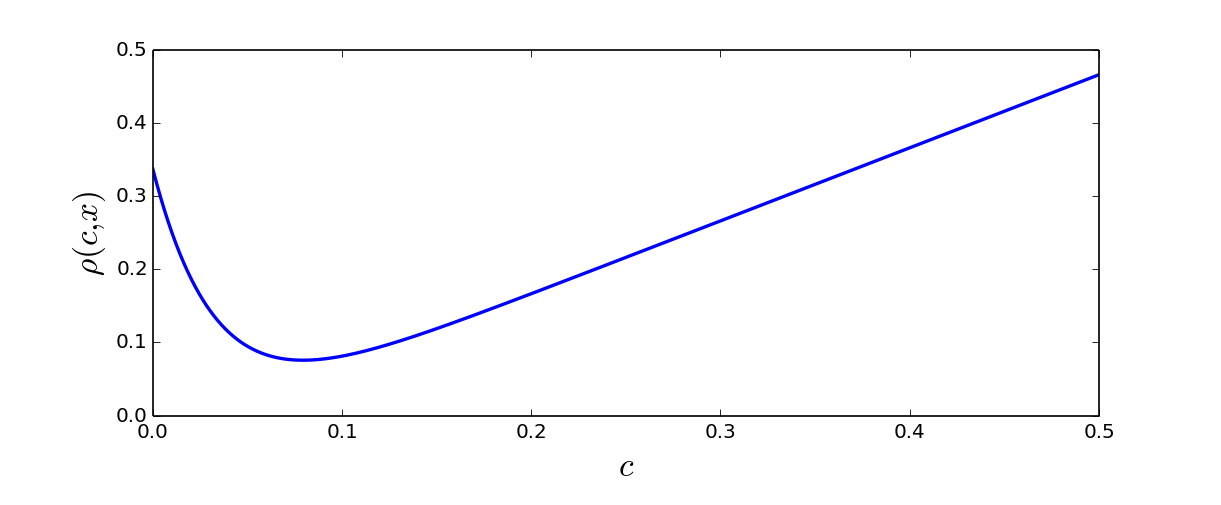
\includegraphics[width=0.85\textwidth]{rho.png}
    % Source: Original work by Jeffrey W. Miller.
  \end{center}
  \caption{Posterior expected loss for the disease prevalence example.}
  \label{figure:rho}
\end{figure}

% \begin{figure}
  % \begin{center}
    % 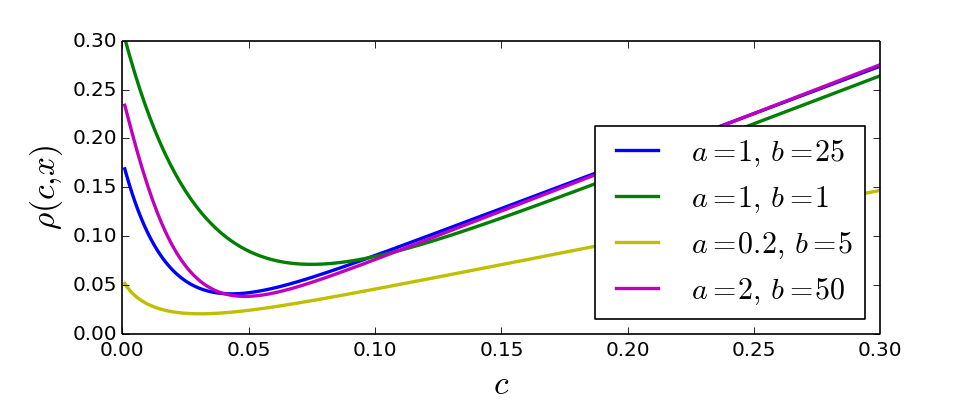
\includegraphics[width=0.8\textwidth]{sensitivity.png}
    % % Source: Original work by Jeffrey W. Miller.
  % \end{center}
  % \caption{Assessing sensitivity to the prior parameters.}
  % \label{figure:sensitivity}
% \end{figure}

\subsubsection*{The Bayes procedure}
\begin{itemize}
\item The Bayes procedure is to minimize the posterior expected loss
$$\rho(c,x) =\E(\ell(\btheta,c)|x) = \int \ell(\theta,c)p(\theta|x)d\theta $$
where $x = x_{1:n}$. We know $p(\theta|x)$ from Equation \ref{equation:Beta-Bernoulli-posterior}, so we can numerically compute this integral for each $c$.
\item Figure \ref{figure:rho} shows $\rho(c,x)$ for our example. To visualize why it looks like this, think about the shape of $\ell(\theta,c)$ as a function of $c$, for some fixed $\theta$---then imagine how it changes as $\theta$ goes from 0 to 1, and think about taking a weighted average of these functions, with weights determined by $p(\theta|x)$.
\item The minimum occurs at $c\approx 0.08$, so under the
    assumptions above, this is the optimal amount of resources to allocate. Note that this makes more sense than naively
    choosing $c=\bar x=1/30 \approx 0.03$, which does not account for uncertainty in $\theta$ and
    the large loss that would result from possible under-resourcing.
%\item (Note: A sensitivity analysis should also be performed to assess how much these results depend on the assumptions. More on this later.)
%\item To assess how sensitive this is to the prior, Figure \ref{figure:sensitivity} shows $\rho(c,x)$ for various choices of $a$ and $b$. A more thorough sensitivity analysis might involve finding the minimizer for all pairs of $a$ and $b$ within some specified ranges, and perhaps also assessing sensitivity to the loss function.
\end{itemize}




%\vspace{20ex}

\subsection{Frequentist risk and Integrated risk}

\begin{itemize}
\item Consider a decision problem in which $S = \btheta$.
\item The \term{risk} (or \term{frequentist risk}) associated with a decision procedure $\delta$ is 
$$ R(\theta,\delta) = \E\big(\ell(\btheta,\delta(X))\mid\btheta =\theta\big),$$
where $X$ has distribution $p(x|\btheta)$.  In other words,
$$ R(\theta,\delta) = \int \ell(\theta,\delta(x))\,p(x|\theta)\,dx$$
if $X$ is continuous, while the integral is replaced with a sum if $X$ is discrete.
\item The \term{integrated risk}  associated with $\delta$ is
$$ r(\delta) = \E(\ell(\btheta,\delta(X)) = \int R(\theta,\delta)\,p(\theta)\,d\theta.$$
\item The diagram in Figure \ref{figure:diagram} (denoting $L = \ell(\btheta,\delta(X))$ for brevity) helps to visualize the relationships between all of these concepts.
\end{itemize}

\begin{figure}
\centering

\begin{tikzpicture}[>=latex] %,text height=1.5ex,text depth=0.25ex]
  \matrix[row sep=-0.5ex,column sep=1ex] {
    & \node (Lt) {Loss}; &  \\
    & \node (L) {$L=\ell(\btheta,\delta(X))$}; &  \\
    & \node (blank1) {}; & \\
    & \node (blank2) {}; & \\
    & \node (blank3) {}; & \\
    & \node (blank4) {}; & \\
    \node (Bt) {Post.\ exp.\ loss}; & & \node (Rt) {Frequentist risk~}; \\ 
    \node (B) {$\E(L\mid X=x)$}; & & \node (R) {$\E(L\mid\btheta=\theta)$}; \\ 
    & \node (blank5) {}; & \\
    & \node (blank6) {}; & \\
    & \node (blank7) {}; & \\
    & \node (blank8) {}; & \\
    & \node (rt) {Integrated risk}; &  \\
    & \node (r) {$\E(L)$}; &  \\
    };
    
    % The diagram elements are now connected through arrows:
    \path[->]
        (L) edge[thick] (Bt)
        (L) edge[thick] (Rt)
        (B) edge[thick] (rt)
        (R) edge[thick] (rt)
;
\end{tikzpicture}

\caption{Visualizing the relationships between different decision-theoretic objects.}
\label{figure:diagram}
\end{figure}


\subsubsection{Example: Resource allocation, revisited}
\label{section:resource-allocation-revisited}

\begin{itemize}
\item The frequentist risk provides a useful way to compare decision procedures in a prior-free way.
\item In addition to the Bayes procedure above, consider two other possibilities: choosing $c = \bar x$ (sample mean) or $c=0.1$ (constant).
\item Figure \ref{figure:procedures} shows each procedure as a function of $\sum x_i$, the observed number of diseased cases. For the prior we have chosen, the Bayes procedure always picks $c$ to be a little bigger than $\bar x$.
\item Figure \ref{figure:risk} shows the risk $R(\theta,\delta)$ as a function of $\theta$ for each procedure. Smaller risk is better. (Recall that for each $\theta$, the risk is the expected loss, averaging over all possible data sets. The observed data doesn't factor into it at all.)
\item The constant procedure is fantastic when $\theta$ is near $0.1$, but gets very bad very quickly for larger $\theta$. The Bayes procedure is better than the sample mean for nearly all $\theta$'s. These curves reflect the usual situation---some procedures will work better for certain $\theta$'s and some will work better for others.
\item A decision procedure is called \term{admissible} if there is no other procedure that is at least as good for all $\theta$ and strictly better for some. That is, $\delta$ is admissible if there is no $\delta'$ such that 
$$R(\theta,\delta')\leq R(\theta,\delta)$$
for all $\theta$ and $R(\theta,\delta')< R(\theta,\delta)$ for at least one $\theta$.
\item Bayes procedures are admissible under very general conditions.
\item Admissibility is nice to have, but it doesn't mean a procedure is necessarily good. Silly procedures can still be admissible---e.g., in this example, the constant procedure $c = 0.1$ is admissible too!
\end{itemize}

\begin{figure}
  \begin{center}
    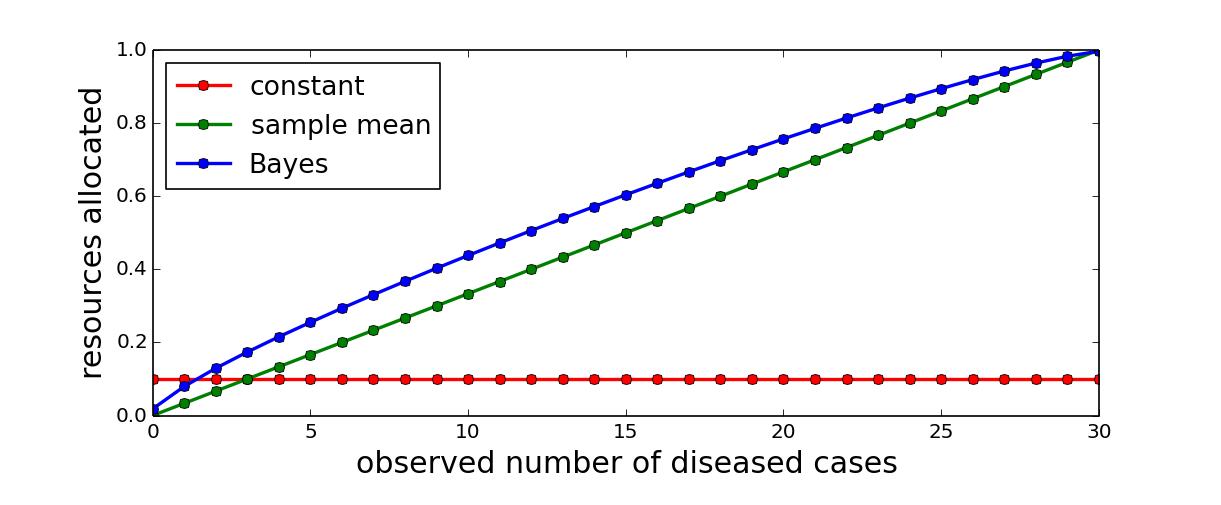
\includegraphics[width=0.85\textwidth]{procedures.png}
    % Source: Original work by Jeffrey W. Miller.
  \end{center}
  \caption{Resources allocated $c$, as a function of the number of diseased individuals observed, $\sum x_i$, for the three different procedures.}
  \label{figure:procedures}
\end{figure}

\begin{figure}
  \begin{center}
    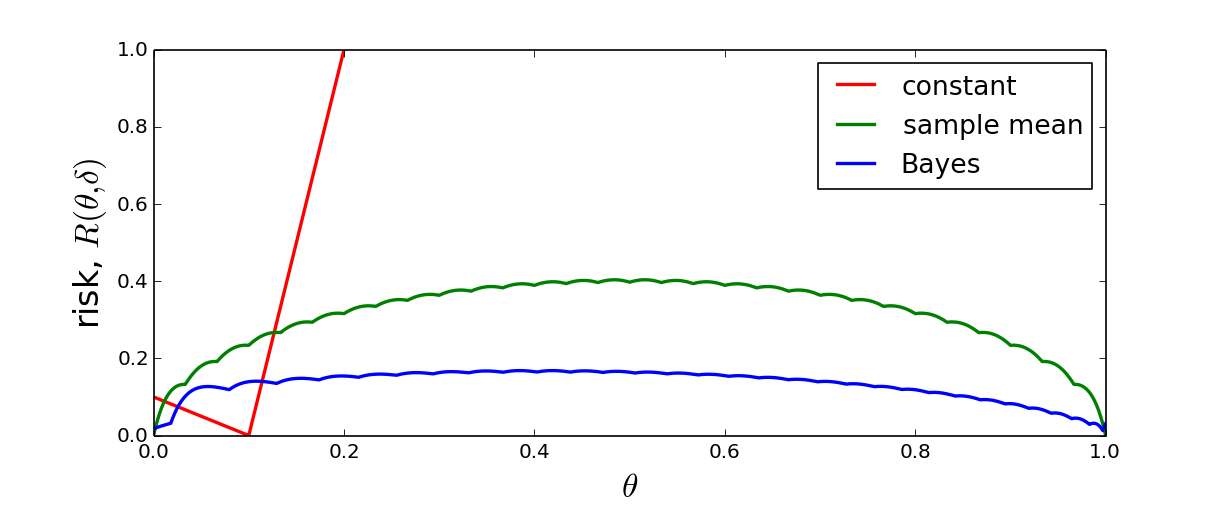
\includegraphics[width=0.85\textwidth]{risk.png}
    % Source: Original work by Jeffrey W. Miller.
  \end{center}
  \caption{Risk functions for the three different procedures.}
  \label{figure:risk}
\end{figure}





%\newpage

\section{Exercises}

\subsubsection*{Gamma-Exponential model}

We write $X\sim\Exp(\theta)$ to indicate that $X$ has the Exponential distribution, that is, its p.d.f.\ is
$$ p(x|\theta) =\Exp(x|\theta) = \theta\exp(-\theta x)\I(x>0). $$
The Exponential distribution has some special properties that make it a good model for certain applications. It has been used to model the time between events (such as neuron spikes, website hits, neutrinos captured in a detector), extreme values such as maximum daily rainfall over a period of one year, or the amount of time until a product fails (lightbulbs are a standard example).

Suppose you have data $x_1,\dotsc,x_n$ which you are modeling as i.i.d.\ observations from an Exponential distribution, and suppose that your prior is $\btheta\sim\Ga(a,b)$, that is,
$$ p(\theta) = \Ga(\theta|a,b) = \frac{b^a}{\Gamma(a)}\theta^{a-1}\exp(-b\theta) \I(\theta>0). $$

\begin{enumerate}
\item Derive the formula for the posterior density, $p(\theta|x_{1:n})$. Give the form of the posterior in terms of one of the distributions we've considered so far (Bernoulli, Beta, Exponential, or Gamma).
\item Now, suppose you are measuring the number of seconds between lightning strikes during a storm, your prior is $\Ga(0.1,1.0)$, and your data is
$$(x_1,\dotsc,x_8) = (20.9, 69.7, 3.6, 21.8, 21.4, 0.4, 6.7, 10.0).$$
Using the programming language of your choice, plot the prior and posterior p.d.f.s. (Be sure to make your plots on a scale that allows you to clearly see the important features.)
\item Give a specific example of an application where an Exponential model would be reasonable. Give an example where an Exponential model would NOT be appropriate, and explain why.
\end{enumerate}


\subsubsection*{Decision theory}

\begin{enumerate}
\setcounter{enumi}{3}
\item Show that if $\ell$ is $0-1$ loss and $S$ is a discrete random variable, then the action $a$ that minimizes the posterior expected loss $\rho(a,x_{1:n})=\E(\ell(S,a)|x_{1:n})$ is the $a$ that maximizes $\Pr(S=a\mid x_{1:n})$.
\item Consider the Beta-Bernoulli model. Intuitively, how would you predict $x_{n+1}$ based on observations $x_1,\dotsc,x_n$? Using your result from Exercise 4, what is the Bayes procedure for making this prediction when $\ell$ is $0-1$ loss?
\item Are there settings of the ``hyperparameters'' $a,b$ for which the Bayes procedure agrees with your intuitive procedure? Qualitatively (not quantitatively), how do $a$ and $b$ influence the Bayes procedure?
\item What is the posterior mean $\E(\btheta|x_{1:n})$, in terms of $a,b$, and $x_1,\dotsc,x_n$? Express this as a convex combination of the sample mean $\bar x=\frac{1}{n}\sum x_i$ and the prior mean (that is, write it as $t \bar x + (1-t) \E(\btheta)$ for some $t\in[0,1]$).
\item Now, consider the loss function and the prior from the example in Section \ref{section:demo}. 
Using the programming language of your choice, reproduce the plot in Figure \ref{figure:rho}. Do the
integrals numerically using a Riemann sum approximation, such as $\int_0^1 f(x)dx \approx \frac{1}{N}\sum_{i = 1}^N f((i-\tfrac{1}{2})/N)$ for a suitably large $N$.
\item Come up with a scenario in which $S$ is discrete but the $0-1$ loss would NOT be appropriate, and give an example of the loss function that would be more suitable.
%\item Show that, in the example of Section \ref{section:resource-allocation-revisited}, the constant procedure is admissible.  Can give more general conditions under which a constant procedure would be admissible?
\end{enumerate}





\section*{References and supplements}

\subsubsection*{Probability basics}
\begin{itemize}
\item Hoff (2009), Sections 2.2--2.6.
\item mathematicalmonk videos, Probability Primer (PP) 2.1 -- 5.5 \\
    \url{https://www.youtube.com/playlist?list=PL17567A1A3F5DB5E4}
\end{itemize}

\subsubsection*{Beta-Bernoulli model}
\begin{itemize}
\item Hoff (2009), beginning of Section 3.1.
\item mathematicalmonk videos, Machine Learning (ML) 7.5 and 7.6 \\ 
    \url{https://www.youtube.com/playlist?list=PLD0F06AA0D2E8FFBA}
\end{itemize}

\subsubsection*{Coin flipping bias}
\begin{itemize}
\item Diaconis, P., Holmes, S., \& Montgomery, R.\ (2007). Dynamical bias in the coin toss. SIAM review, 49(2), 211-235.
\end{itemize}

\subsubsection*{Decision theory}
\begin{itemize}
\item \textit{The Bayesian Choice: From Decision-Theoretic Foundations to Computational Implementation}. Robert, C. P. (2001). Springer Texts in Statistics.
\item \textit{Statistical Decision Theory and Bayesian Analysis}. Berger, J.O. (1985). Springer.
\item mathematicalmonk videos, Machine Learning (ML) 3.1 -- 3.4 and 11.1 -- 11.3 \\ 
    \url{https://www.youtube.com/playlist?list=PLD0F06AA0D2E8FFBA}
\end{itemize}

\subsubsection*{History}
\begin{itemize}
\item \textit{The history of statistics: The measurement of uncertainty before 1900}. Stigler, S.M. (1986). Harvard University Press.
\item Wolfowitz, J. (1952). Abraham Wald, 1902-1950. The Annals of Mathematical Statistics, 1-13.
\item \href{http://youarenotsosmart.com/2014/04/24/yanss-podcast-022-how-we-miss-what-is-missing-and-what-to-do-about-it-with-statistician-megan-price/}{Interesting podcast about Wald}
\end{itemize}




\end{document}







